\chapter{Sorting}
\label{ch:bigo}

\newcommand{\lecnum}{5}
%\newcommand{\lectitle}{Sorting}
\newcommand{\lecturer}{Frank Pfenning, Rob Simmons}

\chapterTAGS{big-o, complexity, correctness, loop-invariant, safety, sorting, testing}
\maketitle

\begin{preamble}
We begin this lecture by discussing how to compare running times of
functions in an abstract, mathematical way.  The same underlying
mathematics can be used for other purposes, like comparing memory
consumption or the amount of parallelism permitted by an algorithm.  We
then use this to take a first look at sorting algorithms, of which
there are many.  In this lecture it will be selection sort because of
its simplicity.
\end{preamble}

\begin{gram}[Learning Goals]
In terms of our learning goals, we will work on:
\begin{description}
\item[Computational Thinking:] Still trying to understand how order
  can lead to efficient computation.  Worst-case asymptotic complexity
  of functions.
\item[Algorithms and Data Structures:] In-place sorting of arrays in
  general, and selection sort in particular.  Big-O notation.
\item[Programming:] More examples of programming with arrays and
  algorithm invariants.
\end{description}
\end{gram}


\section{Big-O Notation}
\label{sec:bigo:bigO}
\TAGS{big-o, complexity}

In the design and analysis of algorithms, we try to make the running time of
functions mathematically precise by deriving so-called \emph{asymptotic
  complexity measures} for algorithms. In addition for wanting mathematical
precision, there are two fundamental principles that guide our mathematical
analysis.
\begin{enumerate}

\item We want an analysis that is \emph{practically useful}. This
  has two consequences.

  First, we observe that the problems we care about are ones that get
  harder as our inputs get bigger, so our definition of Big-$O$
  captures the idea that we only care about the behavior of an
  algorithm \emph{on large inputs}, that is, when it takes a long
  time.  It is when the inputs are large that differences between
  algorithms become really pronounced.

  Second, there is another mathematical concept, Big-$\Theta$, which
  you can read about on your own and which is frequently the concept
  that we actually want to talk about in this class. But computer
  scientists definitely tend to think and talk and communicate in
  terms of Big-$O$ notation. We teach Big-$O$ in part to help you
  communicate with other computer scientists!

\item We want an analysis that is \emph{enduring}. One consequence of
  this is that we want our analysis to be the same even given computers
  that work very different than the ones we use --- in particular, ones
  that are much faster than the ones we use.

  The only way to handle this is to say that we don't care about
  \emph{constant factors} in the mathematical analysis of how long it
  takes our program to run.   In practice,
  constant factors can make a big difference, but they are influenced
  by so many factors (compiler, runtime system, machine model,
  available memory, etc.) that at the abstract, mathematical level a
  precise analysis is neither appropriate nor feasible.

\end{enumerate}
Let's see how these two fundamental principles guide us in the
comparison between functions that measure the running time of an
algorithm.

Let's say we have functions $f$ and $g$ that measure the number of
operations of an algorithm as a function of the size of the input.
For example $f(n) = 3\log n$ measures the number of comparisons performed
in binary search for an array of size $n$, and $g(n) = 3n$
measures the number of comparisons performed in
linear search for an array of size $n$.


The simplest form of comparison would be
\begin{quote}\it
  $f \leq_0 g$ if for every $n \geq 0$, $f(n) \leq g(n)$.
\end{quote}
However, this violates principle (1) because we compare
the values and $f$ and $g$ on all possible inputs $n$.

We can refine this by saying that \emph{eventually},
$f$ will always be smaller than or equal to $g$.  We express
``eventually'' by requiring that there be a number $n_0$
such that $f(n) \leq g(n)$ for all $n$ that are greater
than $n_0$.
\begin{quote}\it
  $f \leq_1 g$ if there is some natural number $n_0$ such that for
  every $n \geq n_0$ it is the case that $f(n) \leq g(n)$.
\end{quote}

This now incorporates the first principle (we only care about the
function on large inputs), but constant factors still matter.  For
example, according to the last definition we have $3n \leq_1 5n$ but
$5n \not\leq_1 3n$.  But if constant factors don't matter, then the
two should be equivalent.  We can repair this by allowing the
right-hand side to be multiplied by a suitable
positive real number.
\begin{quote}
  $f \leq_2 g$ if there is a real constant $c > 0$ and some natural number
$n_0$ such that for every $n \geq n_0$ we have $f(n) \leq c \times g(n)$.
\end{quote}
This definition is now appropriate.

The less-or-equal symbol $\leq$ is already overloaded with many
meanings, so we write instead:
\begin{quote}
  $f \in O(g)$ if there is a real constant $c > 0$ and some natural number
$n_0$ such that for every $n \geq n_0$ we have $f(n) \leq c \times g(n)$.
\end{quote}
This notation derives from the view of $O(g)$ as a set of
functions, namely those that eventually are smaller than a
constant times $g$.\footnote{In textbooks and research papers
you may sometimes see this written as $f = O(g)$ but that
is questionable, comparing a function with a set of functions.}
Just to be explicit, we also write out the definition
of $O(g)$ as a set of functions:
\begin{quote}
  $O(g) = \{ f \mid \mbox{there are $c > 0$ and $n_0$ s.t.\
for all $n \geq n_0$, $f(n) \leq c \times g(n)$} \}$
\end{quote}
With this definition we can check that $O(g(n)) = O(c \times g(n))$.

When we characterize the running time of a function using big-O
notation we refer to it as the \emph{asymptotic complexity} of the
function.  Here, \emph{asymptotic} refers to the fundamental
principles listed above: we only care about the function in the long
run, and we ignore constant factors.  Usually, we use an analysis of
the \emph{worst case} among the inputs of a given size.  Trying to do
\emph{average case} analysis is much harder, because it depends on the
distribution of inputs.  Since we often don't know the distribution of
inputs it is much less clear whether an average case analysis may
apply in a particular use of an algorithm.

The asymptotic worst-case time complexity of linear search is $O(n)$,
which we also refer to as \emph{linear time}.  The worst-case
asymptotic time complexity of binary search is $O(\log n)$,
which we also refer to as \emph{logarithmic time}. \emph{Constant
  time} is usually described as $O(1)$, expressing that the running
time is independent of the size of the input.

Some brief fundamental facts about big-O.  For any polynomial, only
the highest power of $n$ matters, because it eventually comes to
dominate the function.  For example, $O(5n^2 + 3n + 83) = O(n^2)$.
Also $O(\log n) \subseteq O(n)$, but $O(n) \not\subseteq
O(\log n)$.

That is the same as to say $O(\log n) \subsetneq O(n)$, which
means that $O(\log n)$ is a proper subset of $O(n)$, that is,
$O(\log n)$ is a subset ($O(\log n) \subseteq
O(n)$), but they are not equal ($O(\log n) \neq O(n)$).
Logarithms to different (constant) bases are asymptotically the same:
$O(\log_2 n) = O(\log_b n)$ because
$\log_b n = \log_2 n / \log_2 b$.

As a side note, it is mathematically correct to say the worst-case
running time of binary search is $O(n)$, because $\log n \in
O(n)$.  It is, however, a looser characterization than saying that the
running time of binary search is $O(\log n)$, which is also
correct.  Of course, it would be incorrect to say that the running
time is $O(1)$.  Generally, when we ask you to characterize the
worst-case running time of an algorithm we are asking for the tightest
bound in big-O notation.

There is nothing special about the variable $n$. We can use a
different variable, such as $x$, to say $4x + \log_9 x + 2 \in O(x)$,
and we can generalize to multiple variables to say that $2w + 2h^2 + 4
\in O(w + h^2)$. To formalize this, we say that there is a single
constant $c$, but we pick a different starting point $w_0$ and $h_0$
for every variable.

\section{Sorting Algorithms}
\label{sec:bigo:sorts}
\TAGS{sorting}

We have seen in the last lecture that having a sorted array can make
it easier to do search.  This suggests that it may be important to be
able to take an unsorted an array and rearrange it so it's sorted!

There are many different algorithms for sorting: bucket sort, bubble
sort, insertion sort, selection sort, heap sort, etc.  This is
testimony to the importance and complexity of the problem, despite its
apparent simplicity.
In this lecture we discuss selection sort, which is one of the
simplest algorithms.

\clearpage
\section{Selection Sort}
\label{sec:bigo:selection}
\TAGS{sorting}

Selection sort is based on the idea that on each iteration we select
the \emph{smallest} element of the part of the array that has not yet
been sorted and move it to the end of the sorted part at the beginning
of the array.

Let's play this through for two steps on an example array.  Initially,
we consider the whole array (from $i = 0$ to the end).  We write
this as $A\lbrack 0{..}n)$, that is the segment of the array starting at
$0$ up to $n$, where $n$ is \emph{excluded}.
\begin{center}
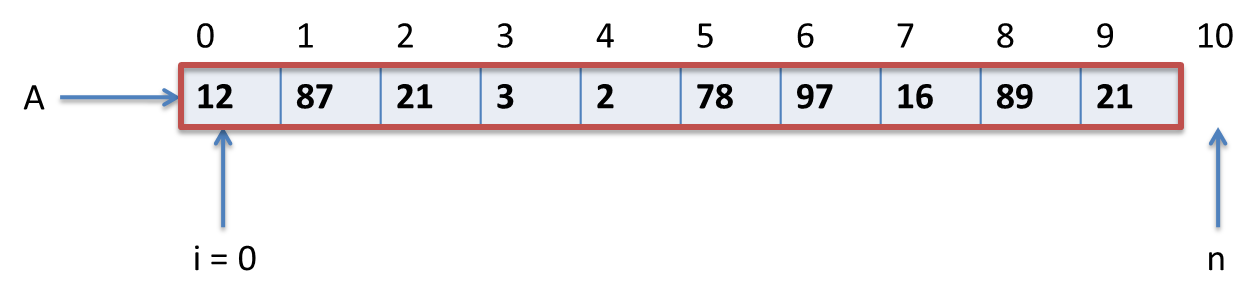
\includegraphics[width=0.85\textwidth]{img/selsort1.png}
\end{center}

We now find the minimal element of the array segment under
consideration ($2$) and move it to the front of the array.  What do we
do with the element that is there?  We move it to the place where $2$
was (namely at $A[4]$).  In other words, we \emph{swap} the first
element with the minimal element.  Swapping is a useful operation when
sorting an array \emph{in place} by modifying it, because the
result of a correct sort must be a permutation of the input.  If swapping is our
\emph{only} operation we are immediately guaranteed that the result is
a permutation of the input.
\begin{center}
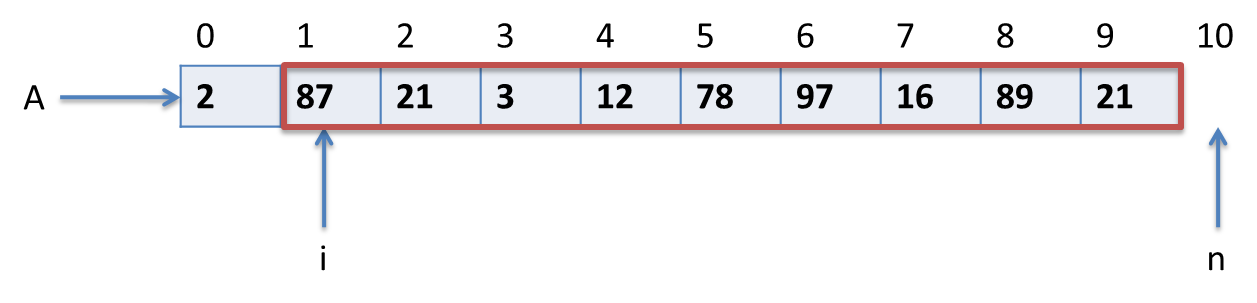
\includegraphics[width=0.85\textwidth]{img/selsort2.png}
\end{center}

Now $2$ is in the right place, and we find the smallest element in the
remaining array segment and move it to the beginning of the segment
($i = 1$).

\clearpage
\begin{center}
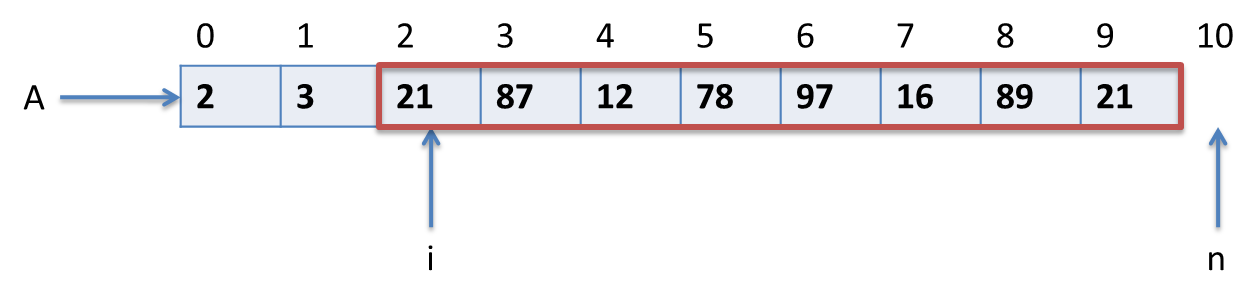
\includegraphics[width=0.85\textwidth]{img/selsort3.png}
\end{center}

Let's pause and see if we can write down properties of the variables
and array segments that allow us to write the code correctly.  First
we observe rather straightforwardly that
$$
0 \leq i \leq n
$$
where $i = n$ after the last iteration and $i = 0$ before the first
iteration.  Next we observe that the elements to the left of $i$
are already sorted.
$$
A\lbrack 0{..}i)\quad \mbox{sorted}
$$
These two invariants are true initially and suffice to imply the
post-condition. However, it won't be possible to prove the correctness
of selection sort because we can't prove that these two invariants, on
their own, are preserved by every iteration of the loop.  We also need
to know that \emph{all} elements to the left of $i$ are less or equal
to \emph{all} element to the right of $i$.  We abbreviate this:
$$
A\lbrack 0{..}i) \leq A\lbrack i{..}n)
$$
saying that every element in the left segment is smaller than or equal
to every element in the right segment.

\clearpage
We summarize the invariants
$$
\begin{array}{l}
   0 \leq i \leq n
\\ A\lbrack 0{..}i)\quad \text{sorted}
\\ A\lbrack 0{..}i) \leq A\lbrack i{..}n)
\end{array}
$$
Let's reason through \emph{without any code} (for the moment), why
these invariants are preserved.
% We also need to make sure they are
% initially true (see the next section).
Let's look at the picture again.
\begin{center}
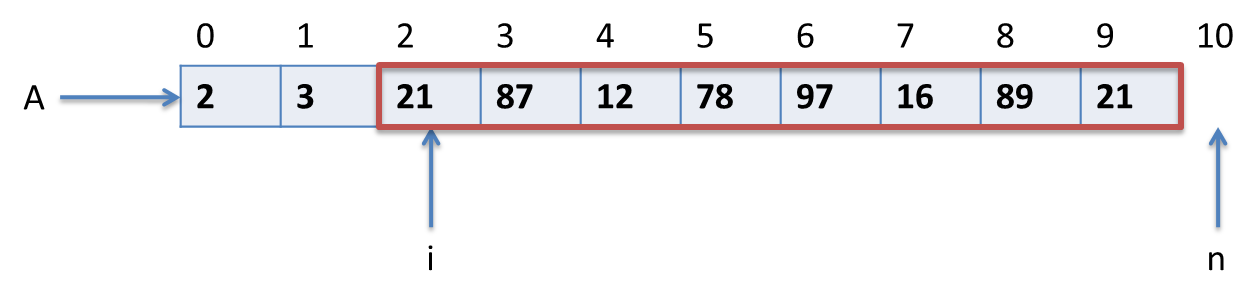
\includegraphics[width=0.85\textwidth]{img/selsort3.png}
\end{center}

In the next iteration we pick the minimal element among $A\lbrack i{..}n)$,
which would be $12 = A[4]$.  We now swap this to $i = 2$ and increment
$i$.  We write here $i' = i+1$ in order to distinguish the old value
of $i$ from the new one, as we do in proofs of preservation of the
loop invariant.
\begin{center}
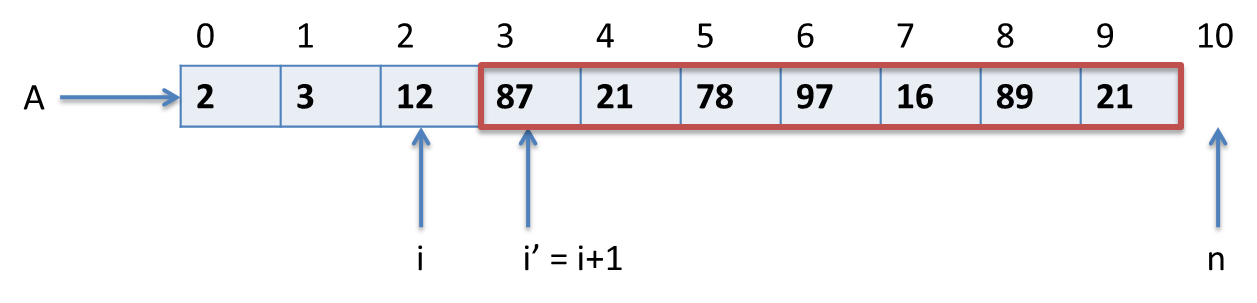
\includegraphics[width=0.85\textwidth]{img/selsort4.png}
\end{center}

Since we only step when $i < n$, the bounds on $i$ are preserved.

Why is $A\lbrack 0{..}i{+}1)$ sorted?  We know by the third invariant that
any element in $A\lbrack 0{..}i)$ is less than or equal to any element in
$A\lbrack i{..}n)$ and in particular the one we moved to $A[i{+}1]$.  And
$A\lbrack 0{..}i)$ was already sorted before by the second invariant.

Why is $A\lbrack 0{..}i{+}1) \leq A\lbrack i{+}1{..}n)$?  We know from the loop
invariant before the iteration that $A\lbrack 0{..}i) \leq A\lbrack i{+}1{..}n)$.  So
it remains to show that $A\lbrack i{..}i{+}1) \leq A\lbrack i{+}1{..}n)$.  But that is
true since $A[i]$ was a minimal element of $A\lbrack i{..}n)$ which is the
same as saying that it is smaller or equal to all the elements in
$A\lbrack i{..}n)$ and therefore also $A\lbrack i{+}1{..}n)$ after we swap the old
$A[i]$ into its new position.

\clearpage
\section{Programming Selection Sort}
\label{sec:bigo:selectioncode}
\TAGS{correctness, loop-invariant, safety, sorting}

From the above invariants and description of the algorithm, the
correct code is simple to write, including its invariants.
The function does not return a value, since it modifies the
given array $A$, so it has declaration:

\begin{lstlisting}[language = {[C0]C}]
void sort(int[] A, int lo, int hi)
//@requires 0 <= lo && lo <= hi && hi <= \length(A);
//@ensures is_sorted(A, lo, hi);
  ;
\end{lstlisting}

We encourage you to now write the function, using the following
auxiliary and contract functions:
\begin{enumerate}
\item%
  \lstinline'is_sorted(A, lo, hi)' which is true if the array segment
  $A\lbrack \mathit{lo}{..}\mathit{hi})$ is sorted.
\item%
  \lstinline'le_seg(x, A, lo, hi)' which is true if $x \leq
  A\lbrack \mathit{lo}{..}\mathit{hi})$ (which means that $x$ is less than
  or equal to all elements in the array segment).
\item%
  \lstinline'le_segs(A, lo1, hi1, lo2, hi2)' which is true if
  $A\lbrack \mathit{lo}_1{..}\mathit{hi}_1) \leq
  A\lbrack \mathit{lo}_2{..}\mathit{hi}_2)$ (which means all elements in the
  first segment are less than or equal to the all elements in the
  second array segment).
\item%
  \lstinline'swap(A, i, j)' modifies the array $A$ by swapping $A[i]$
  with $A[j]$.  Of course, if $i = j$, the array remains unchanged.
\item%
  \lstinline'find_min(A, lo, hi)' which returns the index $m$ of a
  minimal element in the non-empty segment $A\lbrack \mathit{lo}{..}\mathit{hi})$.
\end{enumerate}
Please write it and then compare it to our version on the next
page.

\clearpage
%\lstinputlisting{\code/selsort.c0}
\begin{lstlisting}[language={[C0]C}, numbers=left]
void sort(int[] A, int lo, int hi)
//@requires 0 <= lo && lo <= hi && hi <= \length(A);
//@ensures is_sorted(A, lo, hi);
{
  for (int i = lo; i < hi; i++)
  //@loop_invariant lo <= i && i <= hi;
  //@loop_invariant is_sorted(A, lo, i);
  //@loop_invariant le_segs(A, lo, i, A, i, hi);
  {
    int min = find_min(A, i, hi);
    swap(A, i, min);
  }
}
\end{lstlisting}

At this point, let us verify that the loop invariants are initially
satisfied.
\begin{itemize}
\item%
  $\mathit{lo} \leq i$ and $i \leq \mathit{hi}$ since $i =
  \mathit{lo}$ and $\mathit{lo} \leq \mathit{hi}$ (by the \requires{}
  precondition on line 2).
\item%
  $A\lbrack \mathit{lo}{..}i)$ is sorted, since for $i = \mathit{lo}$ the
  segment $A\lbrack \mathit{lo}..\mathit{lo})$ is empty (has no elements)
  since the right bound is exclusive.
\item%
  $A\lbrack \mathit{lo}{..}i) \leq A\lbrack i{..}\mathit{hi})$ is true since for $i
  = \mathit{lo}$ the segment $A\lbrack \mathit{lo}{..}\mathit{lo})$ has no
  elements.  The other segment, $A\lbrack \mathit{lo}{..}\mathit{hi})$, is
  the whole part of the array that is supposed to be sorted.
\end{itemize}

% We should also verify the assertion we added in the loop body.  It
% expresses that $A[m]$ is less or equal to any element in the segment
% $A[i{..}\mathit{hi})$, abbreviated mathematically as $A[m] \leq
% A[i{..}\mathit{hi})$.  This should be implied by the post-condition of
% the \lstinline'find_min' function.

How can we prove the post-condition (\ensures{}) of the sorting
function?  By the loop invariant $\mathit{lo} \leq i \leq \mathit{hi}$
and the negation of the loop condition $i \geq \mathit{hi}$ we know $i
= \mathit{hi}$.  The second loop invariant then states that
$A\lbrack \mathit{lo}{..}\mathit{hi})$ is sorted, which is the
post-condition.

\clearpage
\section{Auxiliary Functions}
\label{sec:bigo:auxiliary}
\TAGS{correctness, safety}

Besides the specification functions in contracts, we also
used two auxiliary functions: \lstinline'swap' and \lstinline'find_min'.

Here is the implementation of \lstinline'swap'.
%\lstinputlisting[firstline=71,lastline=78]{\code/arrayutil.c0}
\begin{lstlisting}[language={[C0]C}, numbers=left]
void swap(int[] A, int i, int j)
//@requires 0 <= i && i < \length(A);
//@requires 0 <= j && j < \length(A);
{
  int tmp = A[i];
  A[i] = A[j];
  A[j] = tmp;
}
\end{lstlisting}


For \lstinline'find_min', we recommend you follow the method used for
selection sort: follow the algorithm for a couple of steps on a
generic example, write down the invariants in general terms, and then
synthesize the simple code and invariants from the result.  What we
have is below, for completeness.

%\lstinputlisting{\code/findmin.c0}
\begin{lstlisting}[language={[C0]C}, numbers=left]
int find_min(int[] A, int lo, int hi)
//@requires 0 <= lo && lo < hi && hi <= \length(A);
//@ensures lo <= \result && \result < hi;
//@ensures le_seg(A[\result], A, lo, hi);
{
  int min = lo;
  for (int i = lo+1; i < hi; i++)
  //@loop_invariant lo <= i && i <= hi;
  //@loop_invariant lo <= min && min < hi;
  //@loop_invariant le_seg(A[min], A, lo, i);
  {
    if (A[i] < A[min]) {
      min = i;
    }
  }

  return min;
}
\end{lstlisting}


\section{Asymptotic Complexity Analysis}
\label{sec:bigo:bigOanalysis}
\TAGS{complexity, sorting}

Previously, we have had to prove that functions actually terminate.
Here we do a more detailed argument: we do counting in order to
give a big-O classification of the number of operations.  If we have
an explicit bound on the number of operations that, of course, implies
termination.

Assume \(\mathit{lo}=0\) and \(\mathit{hi}=n\) for notational
simplicity.  The loop in function \lstinline'sort' iterates $n$ times,
from $i = 0$ to $i = n-1$.  Actually, we could stop one iteration
earlier, but that does not effect the asymptotic complexity, since it
only involves a constant number of additional operations.

For each iteration of this loop (identified by the value for $i$),
\lstinline'find_min' does a linear search through the array segment to
the right of $i$.  We then do a simple swap.  The linear search will
take $n-i-1$ iterations, and cannot be easily improved since the array
segment $A\lbrack i+1{..}n)$ is not (yet) sorted.  So the total number of
iterations (counting the number of inner iterations for each outer
one)
$$
(n-1) + (n-2) + (n-3) + \cdots + 0 = \frac{n(n-1)}{2}
$$
During each of these iterations, we only perform a constant amount
of operations (some comparisons, assignments, and increments),
so, asymptotically, the running time can be estimated as
$$
O(\frac{n(n-1)}{2}) = O(\frac{n^2}{2} - \frac{n}{2}) = O(n^2)
$$
The last equation follows since for a polynomial, as we remarked
earlier, only the degree matters.

We summarize this by saying that the worst-case running time of
selection sort is quadratic.  In this algorithm there isn't a
significant difference between average case and worst case analysis:
the number of iterations is exactly the same, and we only save one or
two assignments per iteration in the loop body of the \lstinline'find_min'
function if the array is already sorted.

\clearpage
\section{Empirical Validation}
\label{sec:bigo:empirical}
\TAGS{complexity, testing}

If the running time is really $O(n^2)$ and not asymptotically
faster, we predict the following: for large inputs, its running time
should be essentially $c n^2$ for some constant $c$.  If we
\emph{double} the size of the input to $2n$, then the running time
should roughly become $c(2n)^2 = 4(c n^2)$ which means the function
should take approximately 4 times as many seconds as before.

We try this with the function \lstinline'sort_time(n, r)' which generates a
random array of size $n$ and then sorts it $r$ times.  You can find
the C0 code as \lstinline'sort-time.c0' in this lecture's code directory.
We run this code several times, with different parameters.


%\begin{small}
\begin{lstlisting}[language={[coin]C}]
% cc0 selectsort.c0 sort-time.c0
% time ./a.out -n 1000 -r 100
Timing array of size 1000, 100 times
0
0.700u 0.001s 0:00.70 100.0%	0+0k 0+0io 0pf+0w
% time ./a.out -n 2000 -r 100
Timing array of size 2000, 100 times
0
2.700u 0.001s 0:02.70 100.0%	0+0k 0+0io 0pf+0w
% time ./a.out -n 4000 -r 100
Timing array of size 4000, 100 times
0
10.790u 0.002s 0:10.79 100.0%	0+0k 0+0io 0pf+0w
% time ./a.out -n 8000 -r 100
Timing array of size 8000, 100 times
0
42.796u 0.009s 0:42.80 99.9%	0+0k 0+0io 0pf+0w
%
\end{lstlisting}
%\end{small}

Calculating the ratios of successive running times, we obtain
$$
\begin{array}{rrr}
       \mbox{n} & \mbox{Time}  & \mbox{Ratio}
\\ \hline
   1000 & 0.700  &
\\ 2000 & 2.700  & 3.85
\\ 4000 & 10.790 & 4.00
\\ 8000 & 42.796 & 3.97
\end{array}
$$
We see that especially for the larger numbers, the ratio is almost
exactly 4 when doubling the size of the input.  Our conjecture of
quadratic asymptotic running time has been experimentally confirmed.

% \section{Mergesort}

% Both mergesort and quicksort are examples of
% \emph{divide-and-conquer}.  We divide a problem into simpler
% subproblems that can be solved independently and then combine the
% solutions.  As we have seen for binary search, the ideal \emph{divide}
% step breaks a problem into two of roughly equal size, because it means
% we need to divide only logarithmically many times before we have a
% basic problem, presumable with an immediately answer.  Mergesort
% achieves this, quicksort not quite, which presents an interesting
% tradeoff when considering which algorithm to chose for a particular
% class of applications.

% Recall linear search for an element in an array, which is $O(n)$.  The
% divide-and-conquer technique of binary search divides the array in
% half, determines which half our element would have to be in, and then
% proceeds with only that subarray.  An interesting twist here is that
% we \emph{divide}, but then we need to \emph{conquer} only a single new
% subproblem.  So if the length of the array is $2^k$ and we divide it
% by two on each step, we need at most $k$ iterations.  Since there is
% only a constant number of operations on each iteration, the overall
% complexity is $O(\log n)$.  As a side remark, if we divided
% the array into 3 equal sections, the complexity would remain
% $O(\log n)$ because $3^k = (2^{\log_2 3})^k =
% 2^{\log_2{3}k}$, so $\log_2 n$ and $\log_3 n$ only
% differ in a constant factor, namely $\log_2 3$.


% \clearpage
% \section*{Exercises}

% \clearpage
% \bibliographystyle{alpha}
% \bibliography{modal}

% \cleardoublepage
